

\documentclass{beamer}


\usetheme{Madrid}


\title{Gate Problems on Control Systems}

% A subtitle is optional and this may be deleted
\subtitle{EC 2016 Q46}

\author{Piyush Kumar Uttam}


\institute[Indian Institute of Technology,Hyderabad] % (optional, but mostly needed)
{
  \inst{1}%
  Department of Electrical Engineering\\
  Indian Institute of Technology,Hyderabad
 }
% - Use the \inst command only if there are several affiliations.
% - Keep it simple, no one is interested in your street address.

\date{}


\subject{Theoretical Computer Science}

\AtBeginSubsection[]
{
  \begin{frame}<beamer>{Outline}
    \tableofcontents[currentsection,currentsubsection]
  \end{frame}
}




\begin{document}


\begin{frame}
\titlepage
\end{frame}



\begin{frame}{Question}
\begin{block}

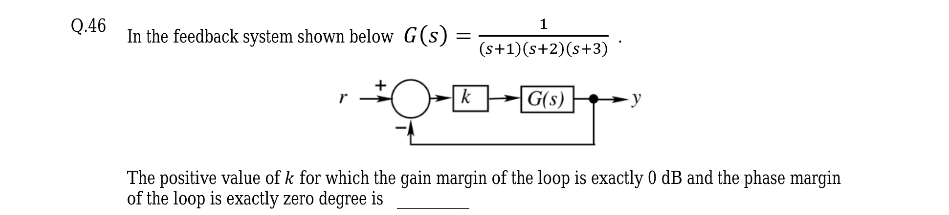
\includegraphics[scale=0.4]{1.png}

\end{block}
\end{frame}
%\begin{frame}
%\tableofcontents
%\end{frame}

\begin{frame}{Theory}

\begin{block}

The gain margin is defined as the change in open-loop gain required to make the closed-loop system unstable. Systems with greater gain margins can withstand greater changes in system parameters before becoming unstable in closed-loop. 

\end{block} \vspace{16pt}
\begin{block}

The phase margin is defined as the change in open-loop phase shift required to make the closed-loop system unstable. The phase margin also measures the system's tolerance to time delay
\end{block} \vspace{16pt}




\end{frame}



\begin{frame}{Technique Description}
\begin{block}

As given in question we see that gain margin is 0 dB and phase margin is 0 degrees. This implies that system is just enough stable and will become destabilized on just small increase in gain. Hence the system is marginbally stable.
\end{block}
\end{frame}
\begin{frame}
\begin{block}


The stability of the system can be checked by Routh-Hurwitz Stability Criterion 
\end{block}

\end{frame}


\begin{frame}{Routh-Hurwitz Stability Criterion}
\begin{block}

Necessary condition for Routh-Hurwitz Stability Criterion: The necessary condition is that the coefficients of the characteristic polynomial should be positive. This implies that all the roots of the characteristic equation should have negative real parts.

Sufficient condition for Routh-Hurwitz Stability Criterion:The sufficient condition is that all the elements of the first column of the Routh array should have the same sign. This means that all the elements of the first column of the Routh array should be either positive or negative.\vspace{16pt}
\includegraphics[scale=0.3]{pic2}
\end{block}

\end{frame}

\begin{frame}
The Routh array for characteristic equation $a_0$s^n+$a_1$s^{n-1}+$a_2$s^{n-2}+.....+$a_{n-1}$s+$a_n$ = 0
\newline
\begin{vmatrix}s^n\\s^{n-1}\\s^{n-2} \\ \vdots \end{vmatrix} \begin{vmatrix}
a_0 & a_2 & a_4 & \cdots \\
a_1 & a_3 & a_5 & \cdots  \\
b_1 & b_2 & b_3 & \cdots \\
\vdots & \vdots & \vdots & \ddots &\vdots 
 \cdots \\ \end{vmatrix} 
 \newline
 where b_1 =\frac{ a_1a_2-a_0a_3}{a_1}  \hspace{5pt} b_2 =\frac{ a_1a_4-a_0a_5}{a_1} \hspace{5pt} c_1=\frac{ b_1a_3-a_1b_2}{b_1}  \hspace{5pt}     c_2=\frac{ b_1a_5-a_1b_3}{b_1} 
\end{frame}

\begin{frame}{Solution}
The Routh array for equation $s^3+6s^2+11s^1+(6+k)$
\begin{table}[]
\begin{tabular}{lllll}
$s^3$ & 1            & 11    &  &  \\
$s^2$ & 6            & (6+k) &  &  \\
$s^1$ & $\frac{66-(6+K)}{6}$& 0     &  &  \\
$s^0$ & $(6+k)$        & 0     &  & 


\end{tabular}
\end{table}
Now since the system is marginally stable therefore $s^1$ row is $\geq$ 0\newline
Hence $\frac{66-(6+K)}{6}$$\geq$0
Hence k=60
\end{frame}
\begin{frame}{Verification using Plots}
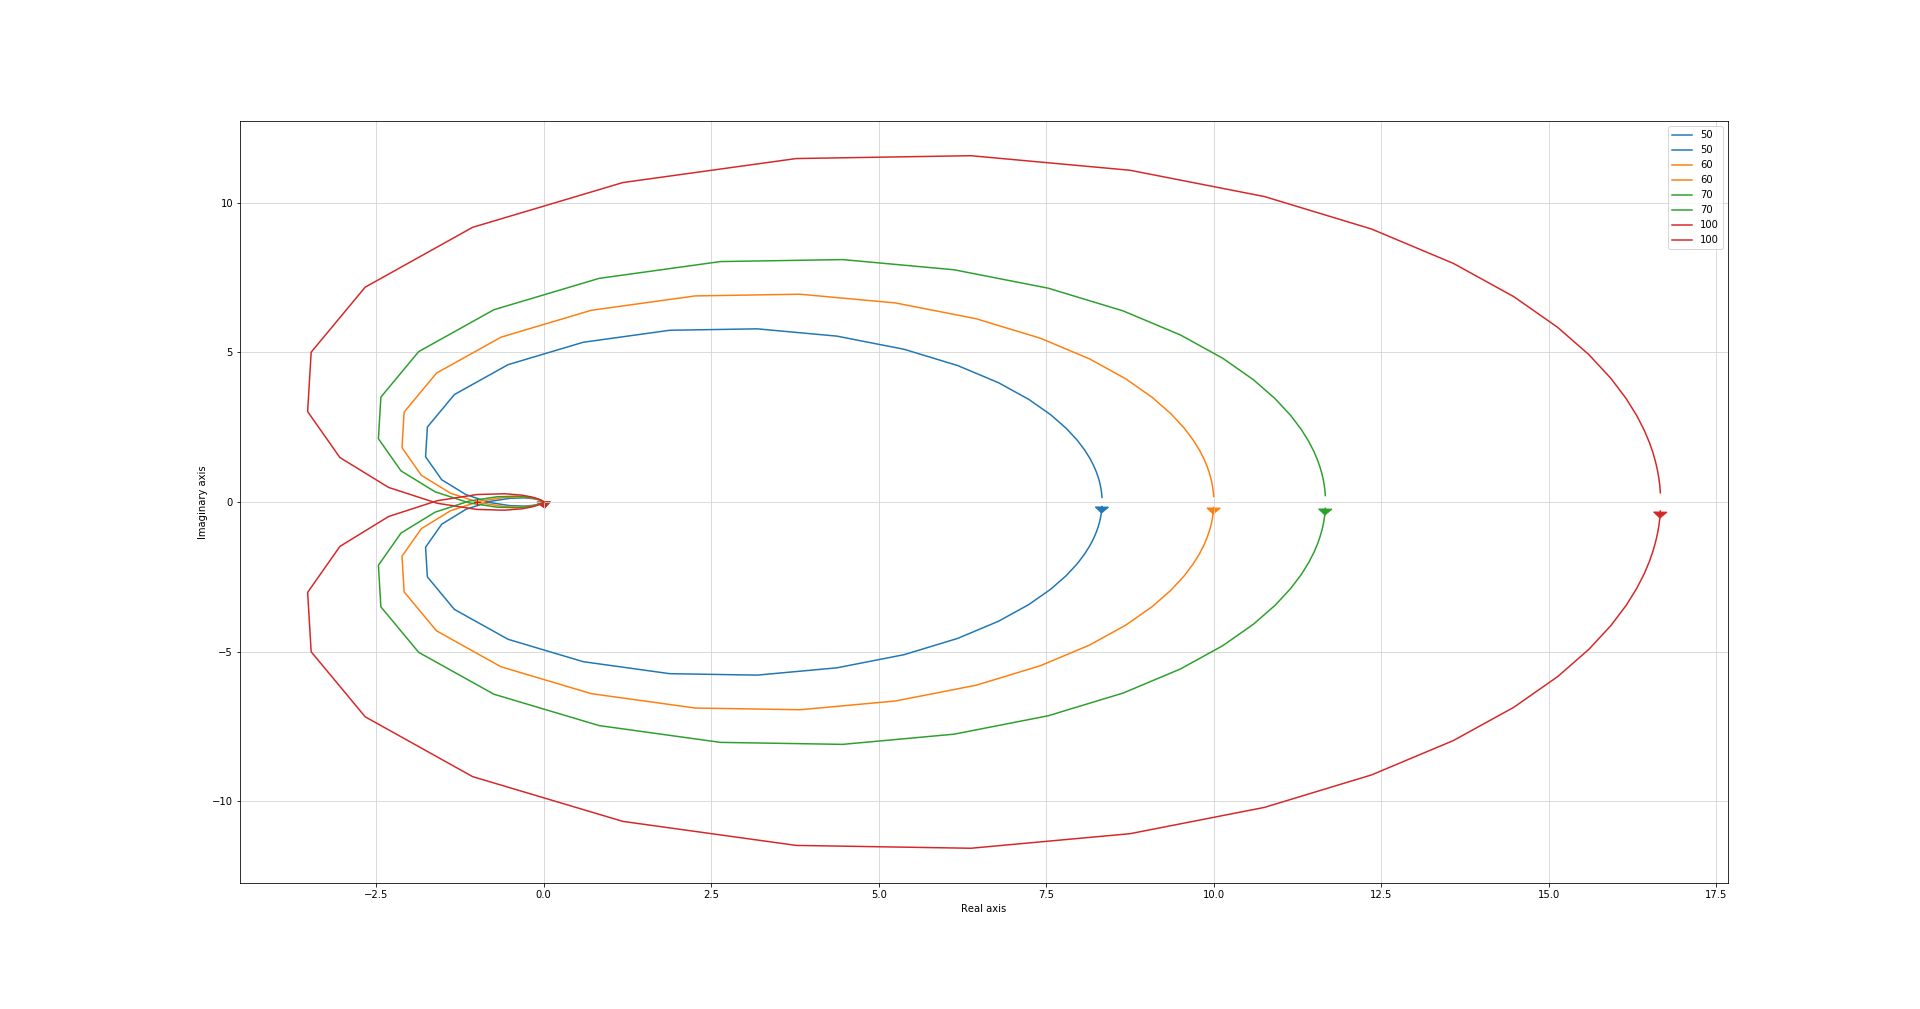
\includegraphics[scale=0.18]{nyq.png}

\end{frame}
\begin{frame}{Verification using Plots}
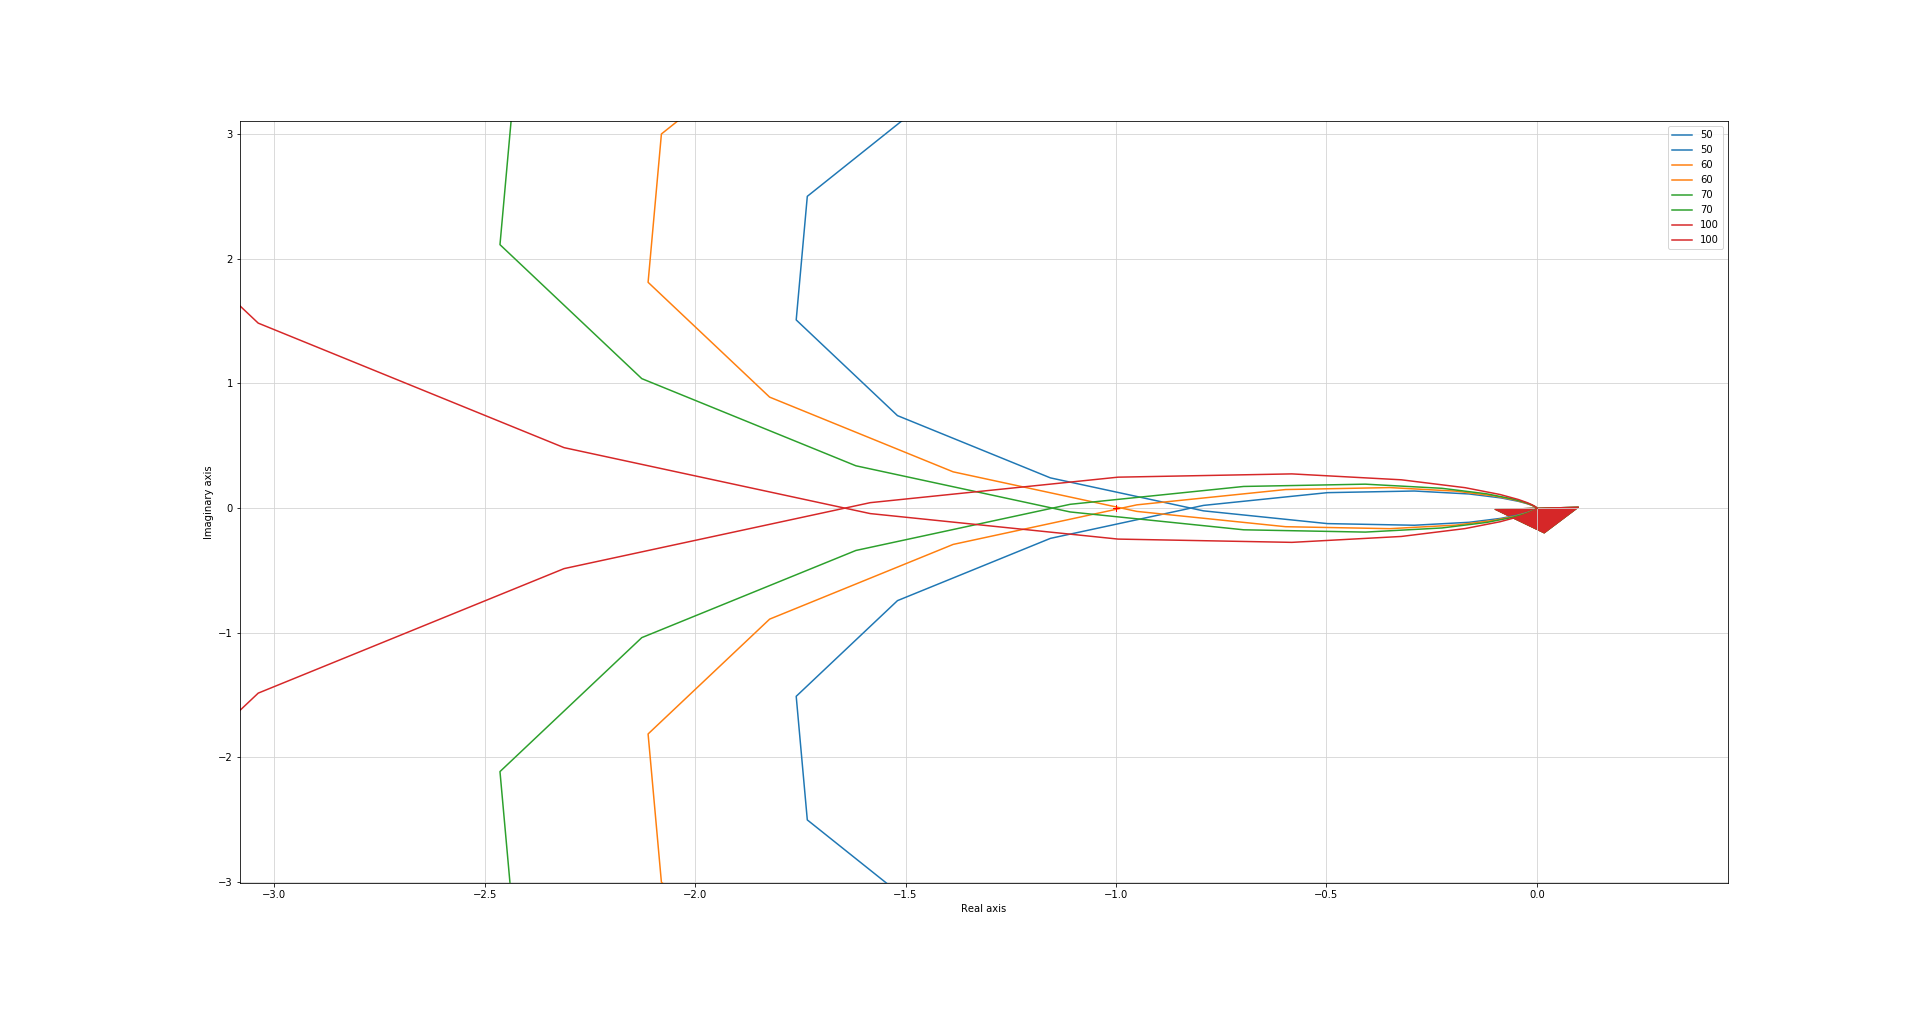
\includegraphics[scale=0.18]{nyq_zoomed.png}

\end{frame}
\end{document}
